% 한국어판 원고 (4쪽, 그림·표·참고문헌 포함).
%
% IEEE Embedded Systems Letters는 영문만 받습니다. 투고 원고는 npuloop_esl.tex이고, 이 파일은 같은
% 내용의 한국어판 -- 읽기용이자 국내 학술대회(대한전자공학회·KIISE·KIPS 등)로 돌릴 때의 출발점입니다.
% 두 파일의 수치는 같은 results/*.json에서 같은 생성기로 나오므로 서로 어긋날 수 없습니다.
%
%   python paper/make_tables.py --lang ko   # -> tab{1,2,3}_rows_ko.tex
%   python paper/make_figs.py   --lang ko   # -> fig{1,2}*_ko.pdf   (한글 글꼴 필요)
%   cd paper && lualatex npuloop_ko && lualatex npuloop_ko
%
% 엔진은 lualatex입니다(한글 조판에 luatexko를 씁니다). pdflatex로는 빌드되지 않습니다.
% IEEEtran measures the Type1 Times family (ptm) while the class itself loads -- before any package
% can run -- and under Unicode (TU) encoding that family does not exist.  Declaring it here, ahead of
% \documentclass, lets the class take its metrics from real Times instead of a silent substitute.
\RequirePackage{fontspec}
\DeclareFontFamily{TU}{ptm}{}
\DeclareFontShape{TU}{ptm}{m}{n}{<->"[texgyretermes-regular.otf]"}{}
\DeclareFontShape{TU}{ptm}{b}{n}{<->"[texgyretermes-bold.otf]"}{}
\DeclareFontShape{TU}{ptm}{bx}{n}{<->ssub*ptm/b/n}{}
\DeclareFontShape{TU}{ptm}{m}{it}{<->"[texgyretermes-italic.otf]"}{}
\DeclareFontShape{TU}{ptm}{b}{it}{<->"[texgyretermes-bolditalic.otf]"}{}
\DeclareFontShape{TU}{ptm}{bx}{it}{<->ssub*ptm/b/it}{}
\documentclass[journal]{IEEEtran}

\usepackage{luatexko}
\setmainfont{TeX Gyre Termes}          % fontspec 기본값(Latin Modern) 대신 IEEEtran과 같은 Times 계열
\setsansfont{TeX Gyre Heros}
\setmonofont{TeX Gyre Cursor}[Scale=MatchLowercase]
% Hangul has no italic and no small caps: IEEEtran's italic subsection heads become Gothic (sans),
% which is how Korean typography marks them, and \textsc falls back to the upright face.
\setmainhangulfont{NanumMyeongjo}[ItalicFont=NanumGothic, BoldItalicFont=NanumGothicBold,
                                  SmallCapsFont=NanumMyeongjo]
\setsanshangulfont{NanumGothic}
\setmonohangulfont{NanumGothicCoding}[Scale=MatchLowercase]
% luatexko draws ASCII punctuation with the Hangul font by default, which turns the periods and
% commas of the English bibliography into CJK-shaped marks.  Korean body text reads fine with
% Latin punctuation, so switch the feature off for the whole document.
\hangulpunctuations=0
% no hyphenation points: "gemm-lowp" across a line break misspells the library.
\hyphenation{gemmlowp}

\usepackage{graphicx}
\usepackage{amsmath}
\usepackage{booktabs}
\usepackage{url}
\usepackage[hidelinks]{hyperref}

\renewcommand{\figurename}{그림}
\renewcommand{\tablename}{표}

\begin{document}

\title{정확도에는 충실하고 텐서에는 충실하지 않다: \\ 모의 양자화와 정수 실행 사이 격차의 연산자별 측정}

% TODO: 투고 전에 저자·소속·연락처를 채울 것.
\author{저자~이름%
\thanks{저자 소속: \textsc{[소속]}, \textsc{[도시, 국가]} (e-mail: \textsc{[이메일]}).}%
\thanks{표와 그림을 재현하는 데 필요한 코드·체크포인트·결과 파일 전부:
\url{https://github.com/sokldjs554/npuloop}.}}

\markboth{npuloop --- 모의 양자화와 정수 실행의 격차}{정확도에는 충실하고 텐서에는 충실하지 않다}
\maketitle

\begin{abstract}
모의(fake) 양자화는 INT8 배포 판단이 내려지는 방식이다. 부동소수점 그래프에 양자화--역양자화 노드를 끼워 넣어
평가하고, 그렇게 나온 정확도를 정수 타깃이 낼 정확도의 대리지표로 삼는다. 이 논문은 그 대리지표가 얼마나 좋은지를
정확도와 텐서에 대해 따로 측정한다. 측정에는 TensorFlow Lite 참조 커널과 비트 단위로 일치하는 정수 엔진을 썼다.
신경망 6종(CNN, 깊이별 합성곱, 분기-연결, 트랜스포머)과 양자화 방식 2종을 전체 테스트셋에서 비교하면 정확도
대리지표는 성립한다. 모의 대 정수 정확도 차이는 모두 $0.20$~\%p 이내이고 12개 $95\%$ 신뢰구간이 전부 0을 포함한다.
텐서는 성립하지 않는다. 출력 코드의 $28.5$--$72.7\%$가 다르고, 이미지의 $95$--$100\%$에서 코드가 최소 하나 다르다.
교사 강제로 분해하면 격차의 출처가 연산자별로 드러난다. 합성곱·선형·풀링은 각각 자기 코드의 $1\%$ 미만에서만
어긋나지만 정수 LayerNorm은 $24.8\%$에서 어긋난다. 시뮬레이터의 LayerNorm을 정수에 충실하게 바꾸면 이 원천은 통째로
사라지지만($24.77\% \rightarrow 0.00\%$) 전파된 출력 코드 불일치는 $72.7\%$에서 $65.7\%$로만 내려간다. 시뮬레이터를
연산자 하나씩 고쳐서 비트 정확한 벡터의 공급원으로 만들 수는 없다는 뜻이다. 아울러 이 대리지표가 가리는 재양자화
선택 하나를 정량화한다. 반올림을 절사로 바꾸면 18개 (모델, 시드, 방식) 조합 전부에서 $0.90$--$3.37$~\%p를 잃으며,
그 손해의 부호는 시드에 강건하지만 크기는 그렇지 않다.
\end{abstract}

\begin{IEEEkeywords}
양자화, 정수 연산, 임베디드 추론, 신경망 처리 장치, 재현성.
\end{IEEEkeywords}

\section{서론}
INT8 가속기에 신경망을 올리는 일은 서로 다른 두 프로그램을 다룬다. 판단에 쓰이는 쪽은 양자화--역양자화(``모의
양자화'') 노드가 삽입된 부동소수점 그래프이고, 그 정확도가 곧 양자화 정확도로 보고된다~\cite{jacob2018,krishnamoorthi2018}.
장치에서 실제로 도는 쪽은 정수 프로그램이다. int8 가중치, int32 누산기, 그리고 고정소수점 곱셈-시프트
재양자화로 이루어진다~\cite{gemmlowp}. 두 프로그램은 서로 바꿔 써도 된다고 가정되며, 정확도에 관한 한 대체로
그렇다~\cite{nagel2021}.

그러나 시뮬레이터에 요구되는 것이 정확도뿐인 것은 아니다. 실리콘 브링업과 컴파일러 검증에는 \textbf{골든 벡터}, 곧
장치가 내놓아야 할 정수 텐서 그 자체가 필요하다. 학습 후 양자화에서 생긴 회귀를 디버깅하려면 \textbf{어느} 연산자에서
격차가 시작되었는지를 알아야 한다. 둘 다 텐서에 관한 질문이고, 시뮬레이터가 이 질문에 답할 수 있는지는 저자가 아는
한 측정된 바 없다.

이 논문은 그것을 측정한다. 기여는 다음과 같다. (i) 모의 양자화와 정수 실행 사이의 격차를, 교사 강제로 떼어 낸
\textbf{국소} 성분(연산자 자신의 정수 연산이 만드는 몫)과 종단간 실행에서 살아남는 \textbf{전파} 성분으로 연산자별
분해하고, 전체 테스트셋에서 대응 표준오차와 함께 보고한다. (ii) 정확도 일치와 텐서 일치가 두 자릿수 규모로 분리되어
있음을 CNN·깊이별 합성곱·분기 연결 구조·트랜스포머와 두 번째 데이터셋에 걸쳐 보인다. (iii) 가장 자연스러운 수리
방법 --- 가장 나쁜 연산자 하나에서 시뮬레이터가 장치의 정수 연산을 쓰게 하는 것 --- 을 직접 시험하여, 국소 격차는
완전히 닫히지만 전파 격차는 거의 닫히지 않음을 보인다. (iv) 정확도 대리지표가 볼 수 없는 재양자화 선택 하나를 시드를
바꿔 가며 측정한다.

\begin{table*}[!t]
\caption{모의 양자화 대 비트 단위로 일치하는 정수 실행, 전체 테스트셋. \textsc{pc}는 채널별 가중치, \textsc{pt}는
텐서별 가중치. $\Delta$는 같은 이미지에서 잰 (정수 $-$ 모의) top-1이며 대응 표준오차를 함께 적었다.
``코드''는 서로 다른 출력 로짓 코드의 비율, ``이미지''는 코드가 하나라도 다른 이미지의 비율이다.}
\label{tab:fidelity}
\centering
\footnotesize
\input{tab1_rows_ko}
\end{table*}

\section{방법}

\subsection{정수 엔진과 그 검증}
보정을 마친 모의 양자화 그래프를 정수 그래프로 내보낸다. int8 가중치, int32 편향, 그리고 출력 채널별 Q31 승수와
시프트로 이루어진다. 실행은 \texttt{MultiplyByQuantizedMultiplier}의 gemmlowp/TensorFlow Lite 의미론을
따르며~\cite{gemmlowp}, 포화 반올림 배증 상위곱과 2의 거듭제곱 반올림 나눗셈을 포함한다. 서로 독립인 두
구현(NumPy와 C++)이 \textbf{모든} 중간 텐서에서 일치할 것을 테스트 스위트가 요구하고, 파이썬을 쓰지 않는 세 번째
C++ 실행기가 직렬화된 파일로부터 같은 코드를 재현한다.

엔진은 자기 자신이 아니라 외부 오라클에 대해 검증한다. TensorFlow Lite의 완전 정수 모델을 가져와 \textbf{그}
스케일·영점·가중치·편향으로 정수 그래프를 세우면, 합성곱과 풀링이 기존 방식의 이중 반올림을 쓰고 완전 연결 계층이
단일 반올림을 쓸 때 $1000/1000$ 이미지의 모든 텐서에서 일치한다. 이 기준이 얼마나 빡빡한지에 대한 눈금으로, 같은
모델에서 TensorFlow Lite 자신의 최적화 델리게이트와 참조 커널은 $1000$장 중 $155$장에서 서로 다른 답을 낸다.

\subsection{국소 불일치와 전파 불일치}
한 장의 이미지에 대해, 모의 양자화 그래프가 노드 $n$에서 만드는 코드를 $f_n$(양자화기 출력을 정수 코드로 환산한 것),
정수 엔진을 종단간으로 돌렸을 때 같은 노드에서 나오는 코드를 $i_n$이라 하자. 노드 $n$의 \textbf{전파} 불일치는
$f_n \neq i_n$인 원소의 비율이다. \textbf{국소} 불일치는 노드 $n$의 정수 커널에 입력으로 모의 양자화 코드를
먹이고(교사 강제) 그 노드의 출력만 비교한 것이다. 국소 불일치는 한 연산자의 정수 연산이 만들어 내는 몫을 떼어 내고,
전파 불일치는 그 몫이 얼마나 멀리 가는지를 보여 준다.

\subsection{통계}
정확도 차이는 대응 표본으로 다룬다. 같은 이미지를 세 번(부동소수점, 모의 양자화, 정수) 평가하고, 이미지별 정답 여부
차이의 평균을 그 표준오차 $s/\sqrt{n}$ 및 $95\%$ Wald 구간과 함께 보고한다. 정확도 열은 모두 전체 테스트셋을
쓴다(CIFAR-10 $10{,}000$장, Imagenette $3{,}925$장). 노드별 분해는 고정된 $250$장 배치(Imagenette는 $125$장)를 쓴다.

\subsection{실험 설정}
CIFAR-10 신경망 5종 --- ReLU를 쓰는 ResNet-20과 SiLU를 쓰는 ResNet-20, MobileNetV2-0.5(깊이별 합성곱), 분기를
연결하는 Inception 계열 CNN, ViT-128/6(어텐션 블록 12개, LayerNorm 13개) --- 과 Imagenette를 $128\times128$로
학습한 ResNet-20 1종을 쓴다. 학습 후 양자화 방식은 둘이다. 채널별 가중치에 비대칭 활성화를 쓰는 방식(\textsc{pc})과
텐서별 가중치를 쓰는 방식(\textsc{pt})이며, 둘 다 학습 이미지 $512$장으로 보정했다. 학습과 평가는 모두 CPU에서
수행했고, 이 논문의 모든 수치는 저장소에 커밋된 결과 파일에서 스크립트가 만들어 낸다.

\section{결과}

\subsection{정확도는 충실하고 텐서는 충실하지 않다}
표~\ref{tab:fidelity}이 핵심 측정이다. 신경망 6종과 방식 2종에 걸쳐 모의 대 정수 정확도 차이의 최댓값은
$0.20$~\%p, $|\Delta|/\mathrm{SE}$의 최댓값은 $1.6$이며, 12개 신뢰구간이 모두 0을 포함한다. 이 표본 크기에서
정확도 대리지표는 정확한 것과 구별되지 않는다. 이미지 단위 top-1 일치율은 $97.9$--$99.7\%$이다.

같은 행이 텐서에서는 어긋난다. 출력 로짓 코드의 $28.5\%$(Inception-32)에서 $72.7\%$(ViT-128/6)가 다르고, 이미지의
$95$--$100\%$에서 코드가 최소 하나 다르다. 트랜스포머가 극단이기는 하나 예외는 아니다. CNN들이 $50$--$63\%$,
입력이 더 큰 Imagenette 모델이 $36\%$에 자리한다. 정확도가 $99\%$ 일치한다는 말은 시뮬레이터가 검증 벡터를 공급할 수
있는지에 대해 아무것도 말해 주지 않는다.

\begin{figure}[!t]
\centering
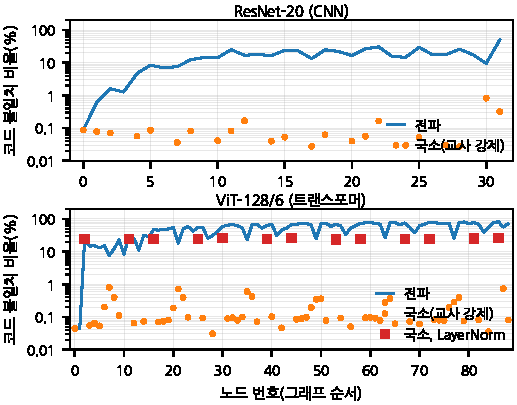
\includegraphics[width=\columnwidth]{fig1_decomposition_ko.pdf}
\caption{노드별 코드 불일치, \textsc{pc} 방식. 국소(교사 강제) 불일치는 LayerNorm을 뺀 모든 연산자에서 $1\%$
미만이고, 전파 불일치는 첫 합성곱에서 시작해 출력의 $50$--$73\%$까지 올라간다. 세로축은 로그 눈금이며, 국소
불일치가 0인 노드(룩업 테이블 활성화, 잔차 덧셈)는 그리지 않았다.}
\label{fig:decomposition}
\end{figure}

\subsection{격차는 어디서 태어나는가}
그림~\ref{fig:decomposition}이 두 성분을 갈라 놓는다. 국소 불일치는 작고 평평하다. 합성곱은 자기 코드의
$0.02$--$0.93\%$, 선형 계층은 $0.03$--$0.96\%$, 평균 풀링은 $0.1$--$2.7\%$(반올림 동점)에서 어긋나며, int8 룩업
테이블 활성화는 정확히 $0\%$이다. 이들은 모두 최하위 비트 $\pm 1$ 수준의 차이다. 반면 전파 불일치는 첫
합성곱에서부터 --- 12개 행 전부에서 첫 격차가 그 노드다 --- 단조롭게 올라가 출력에서 $28$--$73\%$에 이른다.

트랜스포머에는 작지 않은 연산자가 하나 더 있다. 정수 LayerNorm은 부동소수점 대응물과 자기 코드의 $24.8\%$에서
어긋난다(13개 인스턴스 중 최대 $26.2\%$). 정수 구현은 int64 합과 정확한 정수 제곱근으로 정규화하는 반면 시뮬레이터는
float32로 계산한 뒤 격자에 스냅하므로, 대략 원소 넷 중 하나가 반올림 경계의 반대편에 떨어진다. 트랜스포머를 INT8로
옮기는 실무자는 LayerNorm을 가장 먼저 의심해야 한다.

\begin{table}[!t]
\caption{시뮬레이터의 LayerNorm을 정수에 충실하게 바꾼 결과(ViT-128/6, $10{,}000$장). 각 방식의 두 행 사이에서 정수
프로그램은 바뀌지 않았고 시뮬레이터의 LayerNorm만 다르다. 로짓 절대차 평균은 \textsc{pc}에서 $0.119 \rightarrow 0.091$,
\textsc{pt}에서 $0.118 \rightarrow 0.093$으로 줄어든다.}
\label{tab:layernorm}
\centering
\footnotesize
\setlength{\tabcolsep}{4pt}
\begin{tabular}{llcccc}
\toprule
방식 & LayerNorm & 국소(\%) & 코드(\%) & 일치(\%) & $\Delta$ (\%p) \\
\midrule
\textsc{pc} & float32 & 24.77 & 72.7 & 97.93 & $+0.10\pm0.13$ \\
\textsc{pc} & 정수 (13개) & 0.00 & 65.7 & 98.29 & $+0.25\pm0.11$ \\
\textsc{pt} & float32 & 24.76 & 72.6 & 98.07 & $+0.20\pm0.12$ \\
\textsc{pt} & 정수 (13개) & 0.00 & 66.0 & 98.60 & $+0.13\pm0.10$ \\
\bottomrule
\end{tabular}

\end{table}

\subsection{가장 큰 국소 원천을 없애도 격차는 닫히지 않는다}
격차가 연산자별 오차의 합이라면 가장 큰 항을 없앴을 때 그만큼 줄어야 한다. 이를 직접 시험한다. 시뮬레이터의
LayerNorm을, 입력 코드 위에서 엔진의 연산을 그대로 수행하여 구성적으로 비트 단위까지 같은 모듈로 교체하되, 내보낸
정수 프로그램은 그대로 둔다(실험이 이 사실을 단언한다).

표~\ref{tab:layernorm}이 그 결과다. LayerNorm의 국소 불일치는 $24.77\%$에서 정확히 $0.00\%$로 내려가고 로짓 절대차
평균은 약 $23\%$ 개선된다. 그러나 전파된 출력 코드 불일치는 $72.7\%$에서 $65.7\%$로만 움직인다(텐서별은
$72.6\% \rightarrow 66.0\%$). 다른 어떤 연산자보다 두 자릿수 많은 국소 불일치를 책임지던 가장 큰 원천 하나를 없애도
전파 격차의 10분의 1 정도만 회수된다. 남은 것은 개별 국소 불일치가 $1\%$ 미만인 연산자들에서 나온 최하위 비트
$\pm 1$ 사건의 증폭이기 때문이다. 정확도는 어느 방향으로든 대응 표준오차 두 배 안쪽에서 움직이므로 개선으로 읽을 수
없다.

실무적 함의는 분명하다. 비트 정확한 검증 벡터는 정수 구현에서 나와야 한다. 부동소수점 시뮬레이터를 연산자 하나씩
고쳐 나가는 길은 대체재가 되기에는 너무 느리게 수렴한다.

\begin{figure}[!t]
\centering
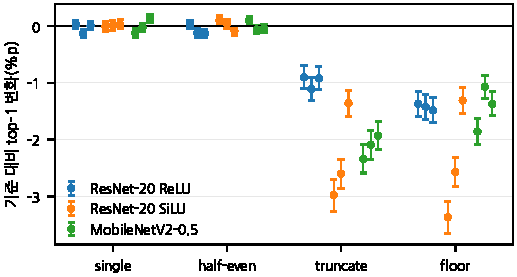
\includegraphics[width=\columnwidth]{fig2_rounding_ko.pdf}
\caption{기준 재양자화 반올림 대비 top-1 변화, 전체 테스트셋, 신경망당 독립적으로 학습한 체크포인트 3개(오차 막대는
대응 표준오차). 편향된 방식들은 모든 조합에서 손해를 보지만, 얼마나 손해인지는 시드마다 다르다.}
\label{fig:rounding}
\end{figure}

\begin{table}[!t]
\caption{기준 구현 대비 반올림 방식의 손해, 시드 3개의 평균 $\pm$ 표준편차(\%p).}
\label{tab:rounding}
\centering
\footnotesize
\setlength{\tabcolsep}{4pt}
\begin{tabular}{lccc}
\toprule
반올림 & ResNet-20 ReLU & ResNet-20 SiLU & MobileNetV2-0.5 \\
\midrule
\texttt{single} & $-0.03\pm0.09$ & $+0.01\pm0.02$ & $-0.00\pm0.13$ \\
\texttt{half\_even} & $-0.07\pm0.09$ & $+0.02\pm0.09$ & $+0.00\pm0.09$ \\
\texttt{truncate} & $-0.98\pm0.12$ & $-2.31\pm0.85$ & $-2.12\pm0.21$ \\
\texttt{floor} & $-1.42\pm0.06$ & $-2.42\pm1.04$ & $-1.43\pm0.40$ \\
\bottomrule
\end{tabular}

\end{table}

\subsection{정확도 대리지표가 가리는 비용}
재양자화의 곱셈-시프트는 반올림 단계로 끝나는데, 구현에 따라 이를 단순 산술 시프트로 바꾸고 싶은 유혹이 있다.
그림~\ref{fig:rounding}과 표~\ref{tab:rounding}은 그 선택을 기준 구현과 비교해 전체 테스트셋에서, 신경망당 독립적으로
학습한 체크포인트 3개로 측정한 것이다.

결과는 둘이다. 첫째, \textbf{부호와 유의성}은 시드에 강건하다. \texttt{truncate}와 \texttt{floor}는 18개 (모델, 시드,
방식) 조합 전부에서 기준보다 나빴고, 그 폭은 $0.90$--$3.37$~\%p, $|\Delta|/\mathrm{SE}$는 $4.4$에서 $11.8$ 사이였다.
반면 단일 반올림과 짝수 반올림 경로는 잡음 범위를 벗어나지 않는다($|\Delta| \leq 0.13$~\%p). 둘째, \textbf{크기}는
그렇지 않다. ResNet-20 SiLU에서 \texttt{truncate}의 손해는 시드 3개에 걸쳐 $1.36$에서 $2.98$~\%p까지 벌어져 시드
표준편차가 효과 크기의 $37\%$에 이르는 반면, ResNet-20 ReLU는 효과의 10분의 1 이내에 머문다. 두 편향 방식 중 어느
쪽이 더 나쁜지는 연산의 성질이 아니라 신경망의 성질이다. ResNet-20 ReLU는 세 시드 모두에서 \texttt{floor}가,
MobileNetV2는 세 시드 모두에서 \texttt{truncate}가 더 많이 잃는다. 반올림 방식의 비용을 시드 하나의 수치로 인용해서는
안 된다.

\section{관련 연구}
MQBench~\cite{mqbench}는 학술 양자화와 배포 가능한 백엔드 사이의 격차를 측정하되 그것을 정확도로 보고한다. 양자화
백서들~\cite{nagel2021,krishnamoorthi2018}은 모의 양자화를 정수 파이프라인의 시뮬레이션으로 다룬다. 배포 툴체인의
계층별 오차 분석은 양자화된 계층이 \textbf{부동소수점} 대응물에서 얼마나 떨어져 있는지를 정량화한다. 여기서의 측정은
종류가 다르다. \textbf{시뮬레이터}가 장치에서 실제로 일어나는 \textbf{정수 실행}에서 얼마나 떨어져 있는지를, 신호 대
잡음비가 아니라 코드 단위로 잰다. 정수만 쓰는 트랜스포머 추론은 정수 LayerNorm과 소프트맥스 커널을 이미
확립했다~\cite{ibert,fqvit}. 그 연산자에 대한 이 논문의 기여는 커널이 아니라, 커널과 시뮬레이터가 얼마나 어긋나는지의
정량화이고 그것을 고치는 것만으로는 충분하지 않다는 증거다. 누산기 폭은 학습 시 제약으로 연구되어 왔다~\cite{a2q}.
여기서 측정하는 축은 그 대신 재양자화 단계의 반올림, 즉 순수한 구현 선택이다.

\section{한계}
신경망은 CIFAR-10 규모에 $128\times128$ Imagenette 모델 하나를 더한 것이다. 따라서 결론은 격차의 구조에 관한 것이지
ImageNet 규모 그래프에서의 정확한 크기에 관한 것이 아니다. 시드 3개는 반올림 축만 덮으며 나머지 측정은 신경망당
체크포인트 하나를 쓴다. 표~\ref{tab:fidelity}의 정확도 비교 12개와 표~\ref{tab:layernorm}의 4개는 다중비교 보정을
하지 않았다(16개 전체에서 $|\Delta|/\mathrm{SE}$의 최댓값은 $2.2$이다). 외부 비트 일치 검증은 합성곱·풀링·완전 연결
계층을 덮고, 깊이별 합성곱·원소별 덧셈·소프트맥스는 덮지 않는다.

\section{재현성}
이 논문의 모든 수치는 커밋된 결과 파일에서 스크립트가 출력하며, 스크립트와 학습된 체크포인트와 그 결과 파일은 모두
공개되어 있다. \texttt{python paper/make\_tables.py}가 표~\ref{tab:fidelity}--\ref{tab:rounding}을,
\texttt{python paper/make\_figs.py}가 그림~\ref{fig:decomposition}--\ref{fig:rounding}을 다시 만든다. 지속적 통합
작업이 커밋마다 생성기를 다시 돌려, 커밋된 표가 결과 파일이 함의하는 표와 다르면 실패시킨다. 측정 자체는
\texttt{experiments/e15\_fidelity.py}(표~\ref{tab:fidelity}과 그림~\ref{fig:decomposition}),
\texttt{e16\_ln\_emulation.py}(표~\ref{tab:layernorm}), \texttt{e14\_rounding\_seeds.py}(그림~\ref{fig:rounding},
표~\ref{tab:rounding})에 있고, 외부 비트 일치 검증은 \texttt{e11\_tflite\_crosscheck.py}이다. 시드를 쓴 측정에는
단서가 하나 붙는다. 이 체크포인트들을 만들 당시 학습기의 시드는 데이터 순서만 통제하고 가중치 초기화는 통제하지
못했으므로, 세 반복은 서로 독립인 표본이지만 같은 명령으로 비트 단위까지 재현되지는 않는다.

\section{결론}
모의 양자화는 INT8 정확도는 잘 맞히고 INT8 텐서는 잘 못 맞히며, 두 사실은 서로 독립이다. 격차를 옮기는 연산자는
하나가 아니다. 개별적으로는 코드의 $1\%$ 미만에서만 어긋나는 연산자들에서 최하위 비트 $\pm 1$ 사건으로 태어나 전파로
자라며, 그래서 가장 나쁜 국소 원천을 없애도 10분의 1밖에 회수되지 않는다. 골든 벡터가 필요한 팀은 외부 기준에 대해
검증된 정수 구현에서 그것을 만들어야 하고, 재양자화의 세부를 바꾸는 팀은 여러 시드에서 측정해야 한다. 그 효과의
크기는 --- 부호와 달리 --- 옮겨 가지 않기 때문이다.

\section*{감사의 글}
% IEEE는 AI 사용 공개를 요구합니다. 실제로 사용한 범위에 맞게 고쳐서 쓰십시오.
저자는 구현의 일부와 실험 스크립트, 그리고 이 원고의 작성에 AI 도구(Claude Code)를 사용했다. 모든 실험은 저자가 직접
실행했고, 보고된 모든 수치는 커밋된 결과 파일에서 커밋된 스크립트가 생성한 것이다.

\IEEEtriggeratref{5}
\begin{thebibliography}{10}
\bibitem{jacob2018} B.~Jacob \emph{et al.}, ``Quantization and training of neural networks for efficient integer-arithmetic-only
inference,'' in \emph{Proc. IEEE/CVF Conf. Comput. Vis. Pattern Recognit. (CVPR)}, 2018, pp. 2704--2713.
\bibitem{krishnamoorthi2018} R.~Krishnamoorthi, ``Quantizing deep convolutional networks for efficient inference: A whitepaper,''
\emph{arXiv:1806.08342}, 2018.
\bibitem{gemmlowp} B.~Jacob \emph{et al.}, ``gemmlowp: a small self-contained low-precision GEMM library,'' 2017. [Online].
Available: \url{https://github.com/google/gemmlowp}
\bibitem{nagel2021} M.~Nagel \emph{et al.}, ``A white paper on neural network quantization,'' \emph{arXiv:2106.08295}, 2021.
\bibitem{mqbench} Y.~Li \emph{et al.}, ``MQBench: Towards reproducible and deployable model quantization benchmark,'' in
\emph{Proc. NeurIPS Datasets and Benchmarks Track}, 2021.
\bibitem{ibert} S.~Kim \emph{et al.}, ``I-BERT: Integer-only BERT quantization,'' in \emph{Proc. Int. Conf. Mach. Learn. (ICML)},
2021, pp. 5506--5518.
\bibitem{fqvit} Y.~Lin \emph{et al.}, ``FQ-ViT: Post-training quantization for fully quantized vision transformer,'' in
\emph{Proc. Int. Joint Conf. Artif. Intell. (IJCAI)}, 2022, pp. 1173--1179.
\bibitem{a2q} I.~Colbert \emph{et al.}, ``A2Q: Accumulator-aware quantization with guaranteed overflow avoidance,'' in
\emph{Proc. IEEE/CVF Int. Conf. Comput. Vis. (ICCV)}, 2023, pp. 16989--16998.
\end{thebibliography}

\end{document}
